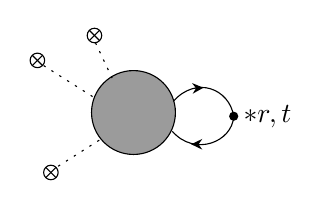
\begin{tikzpicture}[x=0.75pt,y=0.75pt,yscale=-0.5,xscale=0.5]
    %uncomment if require: \path (0,300); %set diagram left start at 0, and has height of 300
    %Shape: Circle [id:dp5242561663737191] 
    \draw  [fill={rgb, 255:red, 155; green, 155; blue, 155 }  ,fill opacity=1 ] (116,155.42) .. controls (116,133.1) and (134.1,115) .. (156.42,115) .. controls (178.74,115) and (196.83,133.1) .. (196.83,155.42) .. controls (196.83,177.74) and (178.74,195.83) .. (156.42,195.83) .. controls (134.1,195.83) and (116,177.74) .. (116,155.42) -- cycle ;
    %Straight Lines [id:da23141236950778143] 
    \draw  [dash pattern={on 0.84pt off 2.51pt}]  (69.83,110.19) -- (118.83,141.19) ;
    %Flowchart: Summing Junction [id:dp8842624208711602] 
    \draw   (70.83,105.19) .. controls (70.83,101.32) and (67.7,98.19) .. (63.83,98.19) .. controls (59.97,98.19) and (56.83,101.32) .. (56.83,105.19) .. controls (56.83,109.05) and (59.97,112.19) .. (63.83,112.19) .. controls (67.7,112.19) and (70.83,109.05) .. (70.83,105.19) -- cycle ; \draw   (68.78,100.24) -- (58.88,110.14) ; \draw   (58.88,100.24) -- (68.78,110.14) ;
    %Flowchart: Summing Junction [id:dp2543754229325399] 
    \draw   (83.83,213.19) .. controls (83.83,209.32) and (80.7,206.19) .. (76.83,206.19) .. controls (72.97,206.19) and (69.83,209.32) .. (69.83,213.19) .. controls (69.83,217.05) and (72.97,220.19) .. (76.83,220.19) .. controls (80.7,220.19) and (83.83,217.05) .. (83.83,213.19) -- cycle ; \draw   (81.78,208.24) -- (71.88,218.14) ; \draw   (71.88,208.24) -- (81.78,218.14) ;
    %Straight Lines [id:da9233967742378848] 
    \draw  [dash pattern={on 0.84pt off 2.51pt}]  (83.83,207.19) -- (124.83,181.19) ;
    %Straight Lines [id:da9217175989381694] 
    \draw  [dash pattern={on 0.84pt off 2.51pt}]  (119.83,88.19) -- (135.83,122.19) ;
    %Flowchart: Summing Junction [id:dp16679591743098143] 
    \draw   (125.83,81.19) .. controls (125.83,77.32) and (122.7,74.19) .. (118.83,74.19) .. controls (114.97,74.19) and (111.83,77.32) .. (111.83,81.19) .. controls (111.83,85.05) and (114.97,88.19) .. (118.83,88.19) .. controls (122.7,88.19) and (125.83,85.05) .. (125.83,81.19) -- cycle ; \draw   (123.78,76.24) -- (113.88,86.14) ; \draw   (113.88,76.24) -- (123.78,86.14) ;
    %Curve Lines [id:da6515102900003924] 
    \draw    (194.83,144.65) .. controls (216.83,119.65) and (248.83,132.52) .. (253,159) ;
    %Curve Lines [id:da6101986878642536] 
    \draw    (193.83,173.52) .. controls (215.83,198.52) and (251.83,183.52) .. (253,159) ;
    %Straight Lines [id:da7630037039793027] 
    \draw    (221,186) -- (215,186) ;
    \draw [shift={(212,186)}, rotate = 360] [fill={rgb, 255:red, 0; green, 0; blue, 0 }  ][line width=0.08]  [draw opacity=0] (10.72,-5.15) -- (0,0) -- (10.72,5.15) -- (7.12,0) -- cycle    ;
    %Straight Lines [id:da6195967819814236] 
    \draw    (216,132) -- (220.84,131.7) ;
    \draw [shift={(223.83,131.52)}, rotate = 176.5] [fill={rgb, 255:red, 0; green, 0; blue, 0 }  ][line width=0.08]  [draw opacity=0] (10.72,-5.15) -- (0,0) -- (10.72,5.15) -- (7.12,0) -- cycle    ;
    %Straight Lines [id:da22490006165025433] 
    \draw    (253,159) ;
    \draw [shift={(253,159)}, rotate = 0] [color={rgb, 255:red, 0; green, 0; blue, 0 }  ][fill={rgb, 255:red, 0; green, 0; blue, 0 }  ][line width=0.75]      (0, 0) circle [x radius= 3.35, y radius= 3.35]   ;
    % Text Node
    \draw (55,151) node [anchor=north west][inner sep=0.75pt]    {$\dotsc $};
    % Text Node
    \draw (260,159) node [anchor=west] [inner sep=0.75pt]   [align=left] {$\vb*{r},t$};
    \end{tikzpicture}